\documentclass[11pt,a4paper,titlepage]{article}

\usepackage{pdflscape}
\usepackage[margin=1in]{geometry}
\usepackage{titling}
\usepackage{graphicx}
\usepackage{titlesec}
\usepackage{datetime}
\usepackage[hidelinks]{hyperref}

\graphicspath{ {./Images/} }

\setcounter{secnumdepth}{4}

\titleformat{\paragraph}
{\normalfont\normalsize\bfseries}{\theparagraph}{1em}{}
\titlespacing*{\paragraph}
{0pt}{3.25ex plus 1ex minus .2ex}{1.5ex plus .2ex}

\newdateformat{monthyeardate}{%
  \monthname[\THEMONTH], \THEYEAR}

\begin{document}
%\title{ \huge Functional Requirements for the SAMBUG}

\begin{titlepage}
	
	
	\begin{center}
		\vspace*{-3cm}
  		\makebox[\textwidth]{
\includegraphics[width=\paperwidth]{sambug}}
	\end{center}
	
	%
\includegraphics[width=\paperwidth]{sambug}
	
    \vspace*{2cm}
      \Huge \textbf {SAMBUG}\\
      
    \vspace*{-0.5cm}
	  \huge \textbf {Functional Requirements}\\
	  \hfill\\
	\vspace*{-0.5cm}  
      
\includegraphics[scale=0.2]{logo}\hfill
	
\includegraphics[scale=0.2]{sambug_logo}
         
    \vskip2cm
          
    \large \textbf{\monthyeardate\today}
  
    \vfill
\begin{tabular}{lr}
        	Abrie van Aardt&13178840\\
		Werner Mostert&13019695\\
		Kale-ab Tessera&13048423\\
		Keagan Thompson&13023782\\
		Michelle Swanepoel&13066294\\
	\end{tabular}
\end{titlepage}
	
%\author
%{     
%	Abrie van Aardt 13178840\\
%	Werner Mostert 13019695\\
%	Kele-ab Tessera 13048423\\
%	Keagan Thompson 13023782\\
%	Michelle Swanepoel 13066294\\
%}
    
%\date{\textbf{May 2015}}

%\maketitle

\tableofcontents

\pagebreak


% Put all images in images folder - Please use PNG's not Jpegs
% Preferably create separate file for your domain - just like with the use cases
\pagebreak


\section{Background}
South Africa is currently the largest producer of macadamia nuts in the world. One of the main production and quality limiting factors is the incidence of stink bug damage. 
\\Accurate timing of chemical sprays rely on accurate scout data and economic threshold levels of the insect pests in an orchard. However, scouting for these pests has
a major shortfall, namely the accurate identification of pests, despite efforts to train growers and scouts by various means.\\
Area wide control of pests and diseases is a concept that has been considered, but with the lack of scout data from across and within growing regions it is impossible to make such recommendations. \\

\section{Vision}
An innovative approach to handling the management and acquisition of scout data is to develop a smartphone application that is able to identify specific hemipteran species by making use of the built-in camera of the smartphone. This application makes use of the smartphone’s built-in GPS to perform geotagging and uploading information to a central database. In addition to the data management, one of the primary goals is to supply data mining methods on historical data as obtained via the smartphone application. A visual representation of said data is therefore made available in a dynamic and easy way for the every day farmer and researcher.

\section{Scope}
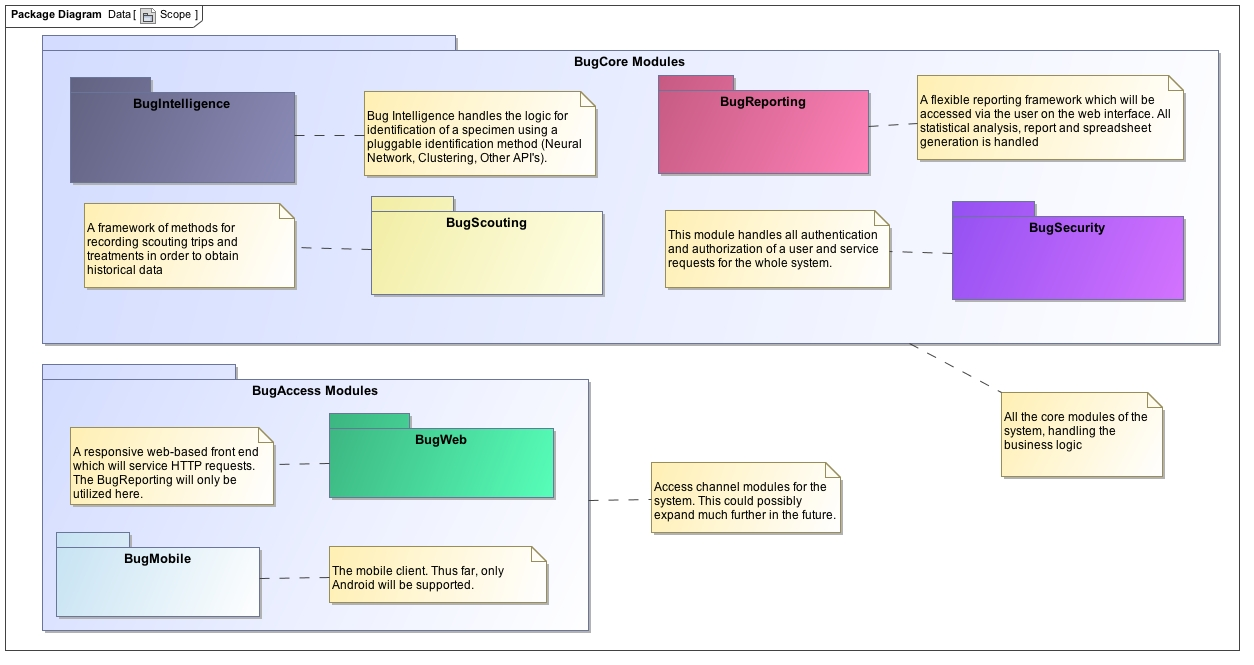
\includegraphics[width=\linewidth]{scope}

%\section{Architecture requirements}
%	\subsection{Access channel requirements}
%	\subsection{Quality requirements}
%	\subsection{Integration requirements}
%	\subsection{Architecture constraints}
\section{Functional Requirements and Application Design}
	\subsection{Domain Model}
		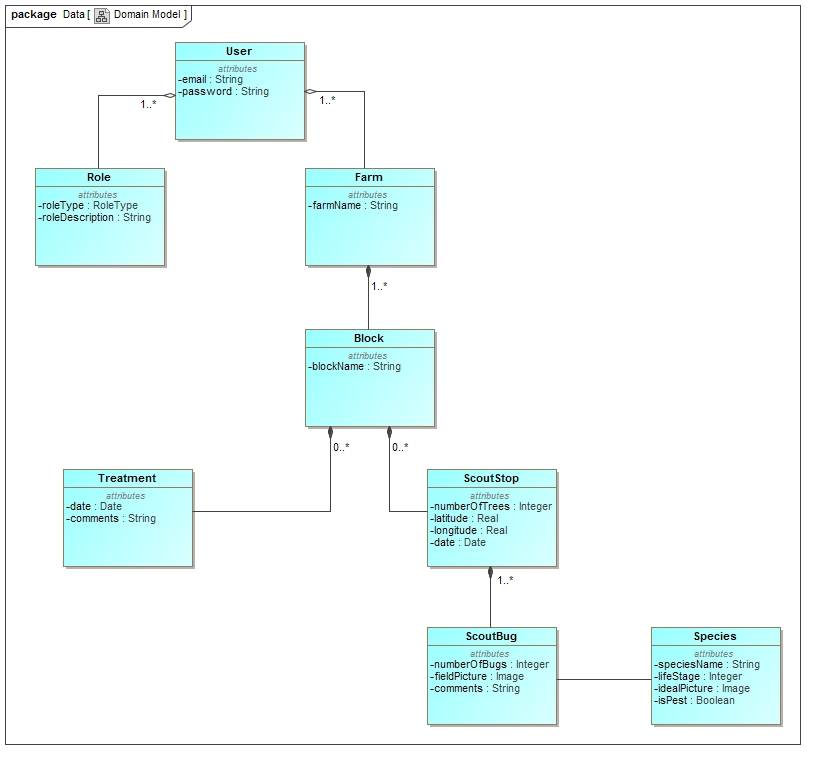
\includegraphics[width=\linewidth]{DomainModel}
%------------------------------------------------------------------------------------------%

	\subsection{BugScouting}
		The BugScouting module has the following functionality:
		\begin{enumerate}
			\item It provides the functionality for a user to be able to enter data related to a scouting trip - entering data such as the number of trees scouted, the number of bugs per tree and the different kind of bugs specified. After this data has been entered, a summary should be displayed for the user.
			\item It provides the ability for a user to record the details related to spraying, such as the date of spraying and the specific block that was sprayed.
		\end{enumerate}

		In many ways this module may be regarded as the "core" functionality of the system. This encompasses the main purpose of the system.
		\subsubsection{Module Scope}
		The scope of the \textit{BugScouting} module is shown below:\\
		\hfill\\
		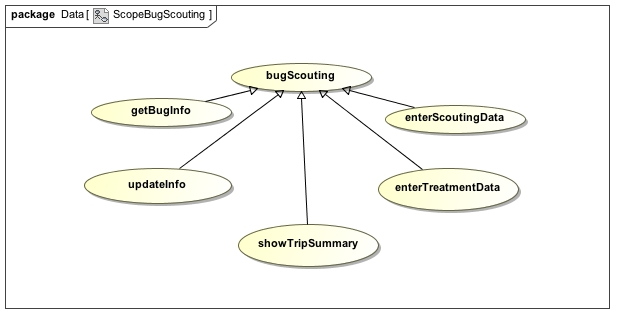
\includegraphics[width=\linewidth]{ScopeBugScouting}
		
		\subsubsection{Use Cases}
		The concrete use cases for the \textit{BugScouting} module follow:
		\paragraph{getBugInfo \dotfill [Priority - Medium]}
		This use case uses the BugIntelligence module to retrieve information on a specific specimen which will be used to display to the user a "wiki" like piece which has the purpose of informing the user.\\\hfill\\
		The Service Contract for the \textit{getBugInfo} use case is shown below:\\\hfill\\
		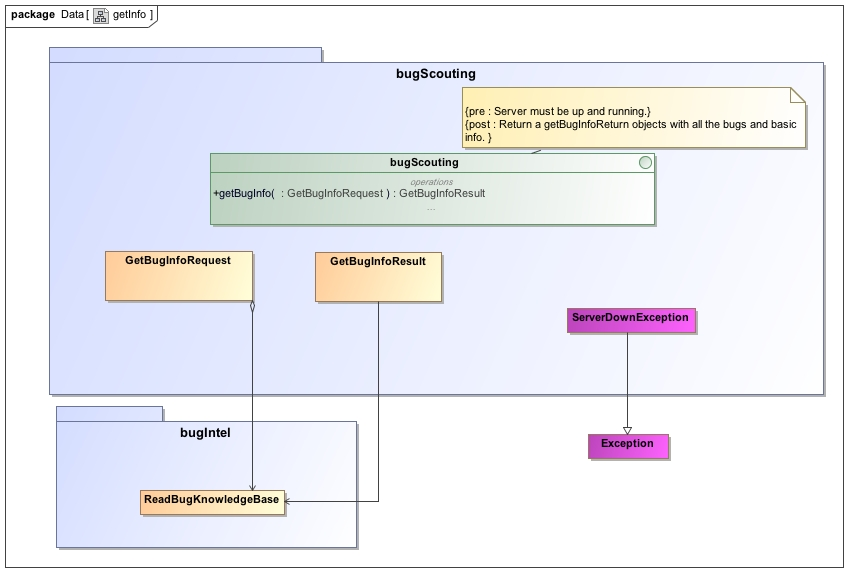
\includegraphics[width=\linewidth]{getInfo}
		
		\paragraph{updateInfo \dotfill [Priority - Medium]}
		The objective of this use case is to provide functionality to retrieve updated bug information and identification method updates.\\\hfill\\
		The Service Contract for the \textit{getBugInfo} use case is shown below:\\\hfill\\
		\includegraphics[width=\linewidth]{updateInfo}
		
		\paragraph{showTripSummary \dotfill [Priority - High]}
		After completing a full scouting trip, this use case should provide a summary of the entire scouting trip. One scouting trip may consist of many scouting stops and each scout stop may include the finding of various bugs. The averages for the scouting trip data is used in the summary.\\\hfill\\
		The Service Contract for the \textit{showTripSummary} use case is shown below:\\\hfill\\
		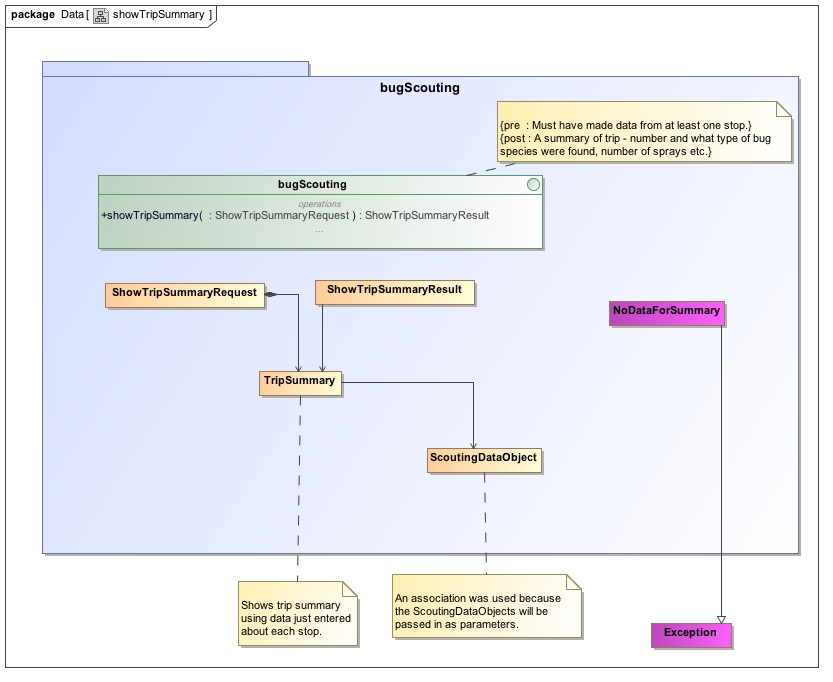
\includegraphics[width=\linewidth]{showTripSummary}
		
		\paragraph{enterTreatmentData \dotfill [Priority - Critical]}
		This use case is for entering data related to spraying chemicals (pesticide). This allows for the type of chemical, the date and the block or orchard number to be recorded.\\\hfill\\
		
		The Service Contract for the \textit{enterTreatmentData} use case is shown below:\\\hfill\\
		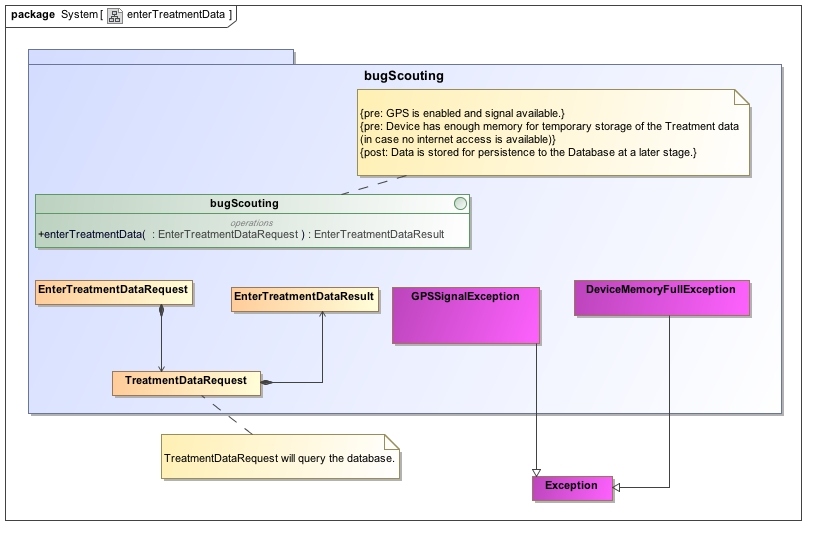
\includegraphics[width=\linewidth]{EnterTreatmentData}
		
		\paragraph{enterScoutingData \dotfill [Priority - Critical]}
		This is the core use case of this module. This use case allows entering data related to a scouting stop. Data captured should include the number of trees observed, the number of bugs encountered and the block number where the scouting took place. After entering the data, the specimen should be identified (classified), either manually or automatically, before successfully submitting it for persistence.\\\hfill\\
		The Service Contract for the \textit{enterScoutingData} use case is shown below:\\\hfill\\
		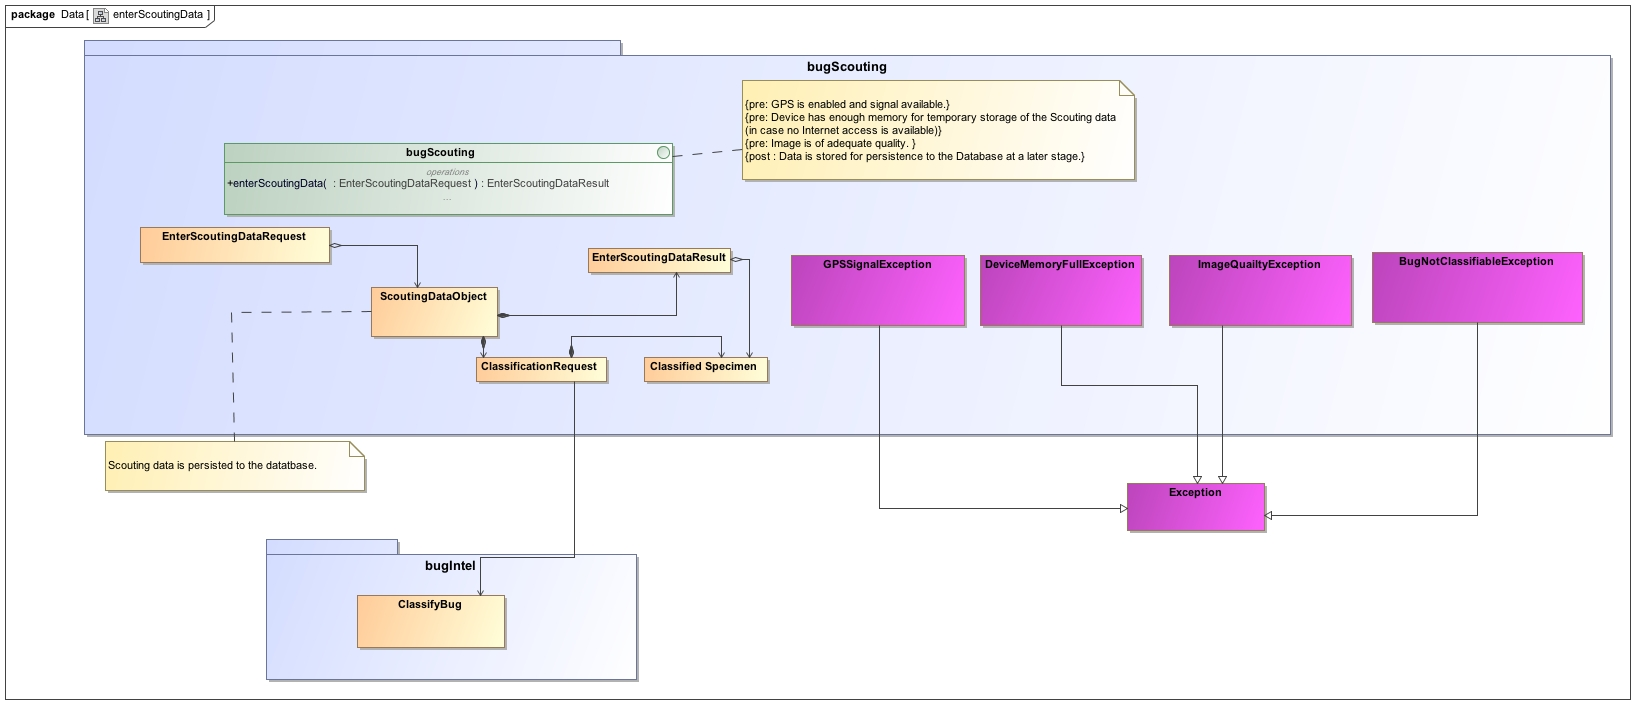
\includegraphics[width=\linewidth]{enterScoutingData}
		The Process Specification for the \textit{enterScoutingData} use case is shown below:\\\hfill\\
		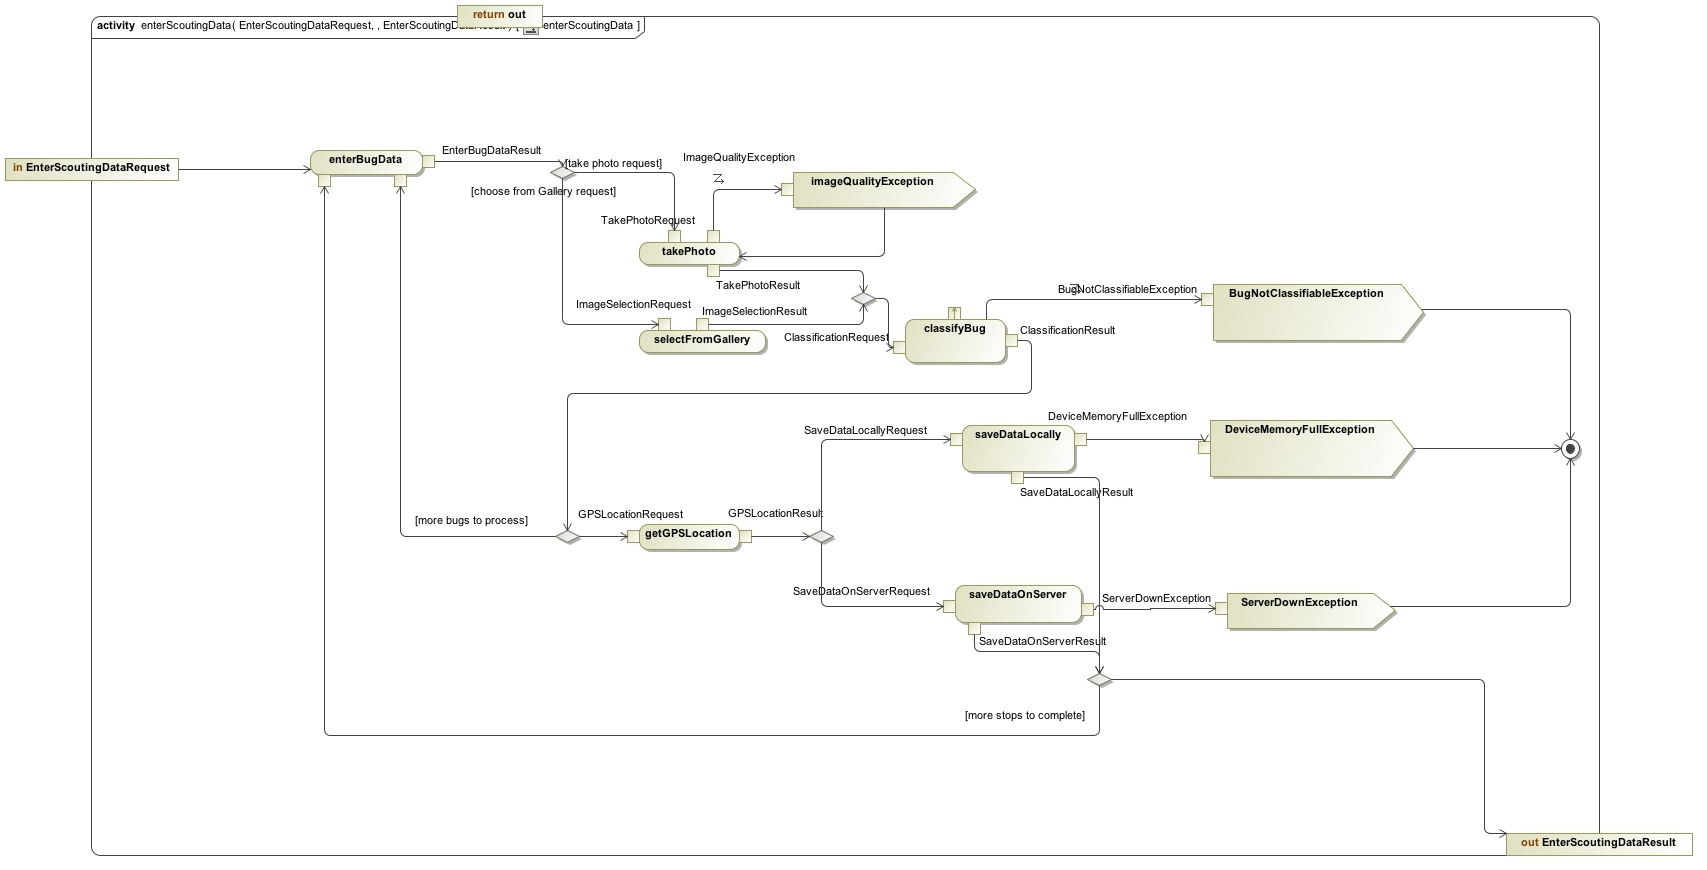
\includegraphics[width=\linewidth]{enterScoutingDataPS}
		
		
		
		
%------------------------------------------------------------------------------------------%	
	
	\subsection{BugIntelligence}
		The BugIntelligence module has the following functionality:
		\begin{enumerate}		
			\item It provides a pluggable method to classify a specimen according to species and life stage.
			\item It provides an interface which can be used to obtain information related to any specific specimen which is identifiable by the system
			\item It provides CRUD(Create Read Update Delete) functionality for bug information for specimens identifiable by the identification method
		\end{enumerate}
		\subsubsection{Module Scope}
		The scope of the \textit{BugIntelligence} module is shown below:\\
		\hfill\\
		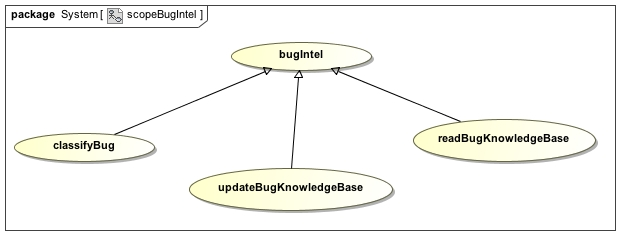
\includegraphics[width=\linewidth]{scopeBugIntel}
		\subsubsection{Use Cases}
		The concrete use cases for the \textit{BugIntelligence} module follow:
		
		\paragraph{classifyBug \dotfill [Priority - Critical]}
		This use case supplies a method to classify the bug according to life stage and species. The classification method used is pluggable.\\\hfill\\
		The Service Contract for the \textit{classifyBug} use case is shown below:\\\hfill\\
		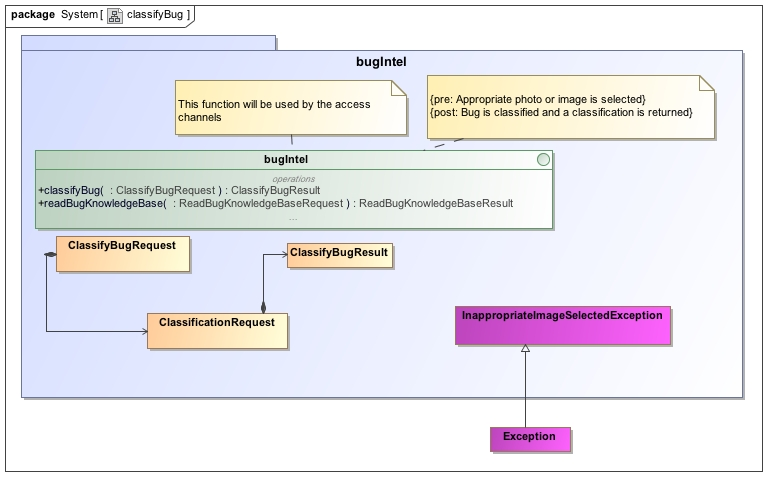
\includegraphics[width=\linewidth]{classifyBug}
		
		The Process Specification for the \textit{classifyBug} use case is shown below:\\\hfill\\
		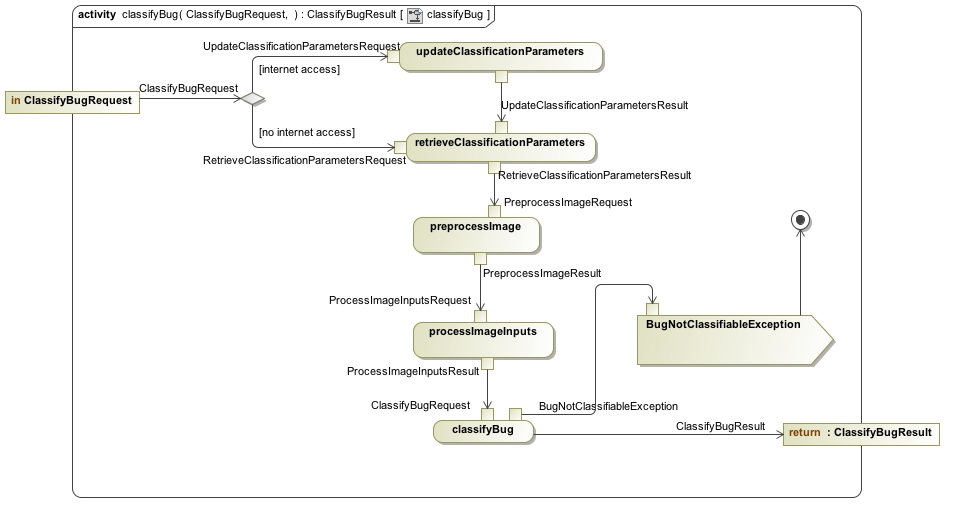
\includegraphics[width=\linewidth]{classfyBugPS}
		
		\paragraph{updateBugKnowledgeBase \dotfill [Priority - Low]}		
		This use case provides the functionality to edit the information used for classification. As in the example of a neural network being used as a classification method, the training examples may be edited.		
		The Service Contract for the \textit{updateBugKnowledgeBase} use case is shown below:\\\hfill\\
		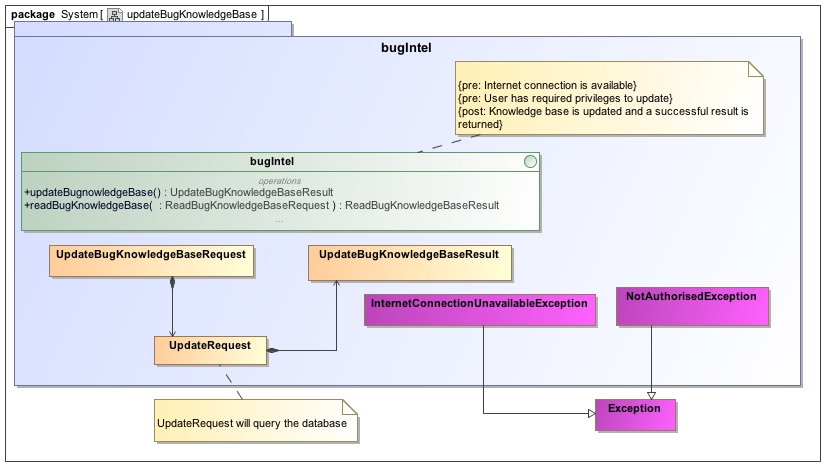
\includegraphics[width=\linewidth]{updateBugKnowledgeBase}
		
		\paragraph{readBugKnowledgeBase \dotfill [Priority - Critical]}
				This use case provides the functionality to get the information used for classification. As in the example of a neural network being used as a classification method, the training examples may be retrieved.	
		The Service Contract for the \textit{readBugKnowledgeBase} use case is shown below:\\\hfill\\
		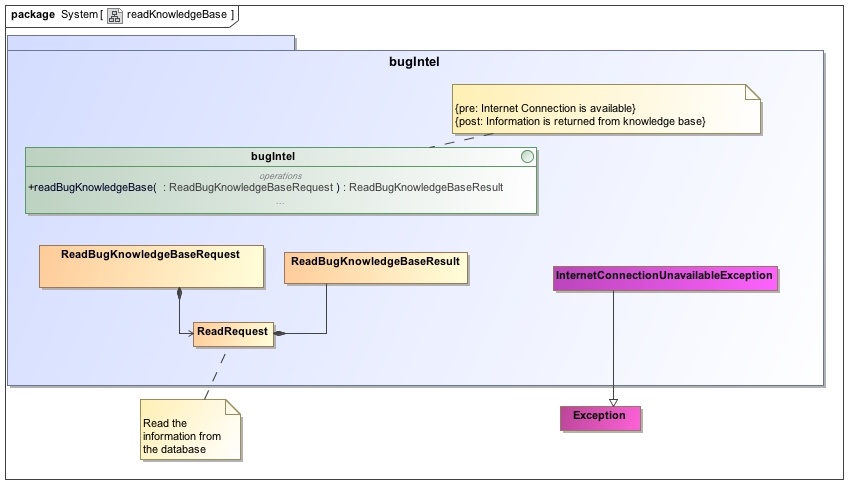
\includegraphics[width=\linewidth]{readKnowledgeBase}
		
		
%------------------------------------------------------------------------------------------%		
	\subsection{BugSecurity}
	The BugSecurity module allows the following functionality:
	\begin{enumerate}
		\item It provides functionality related to user accounts and user roles in order to login, register and recover your account within the capacity of a user role.
		\item It provides functionality to determine whether a specific service request should be allowed.
	\end{enumerate}
		\subsubsection{Module Scope}
		The scope of the \textit{BugSecurity} module is shown below:\\
		\hfill\\
		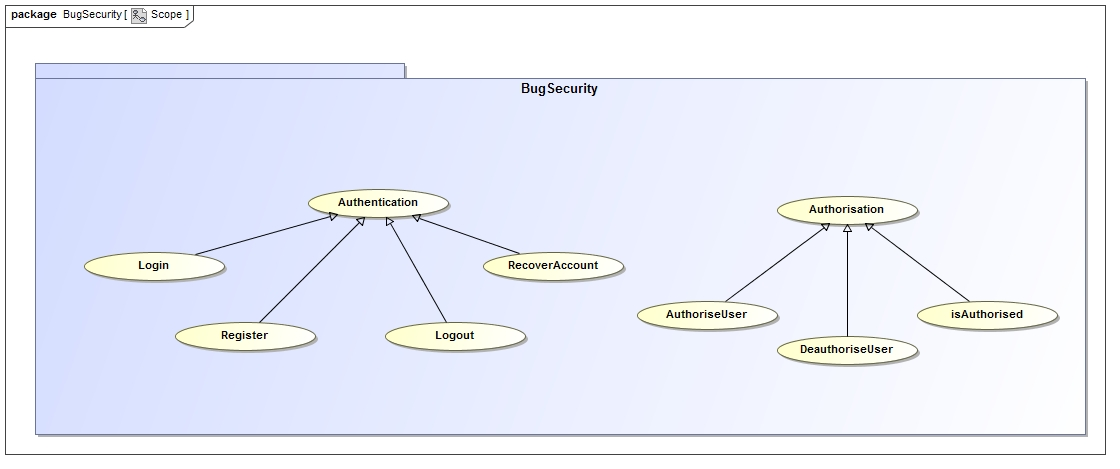
\includegraphics[width=\linewidth]{SecurityScope}
		\subsubsection{Use Cases}
		The concrete use cases for the \textit{BugSecurity} module follow:
		
		\paragraph{login \dotfill [Priority - Critical]}
		This use cases allows one to login with username and password credentials which will be validated and thus allowing the user to be authenticated.\\\hfill\\
		The Service Contract for the \textit{login} use case is shown below:\\\hfill\\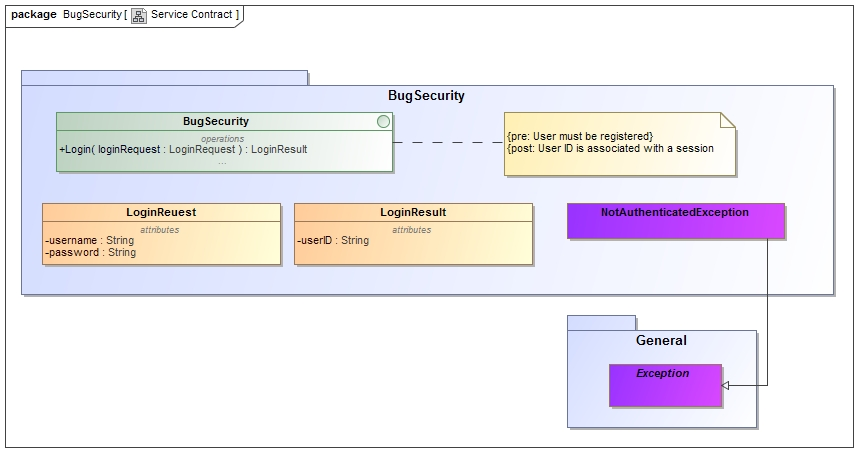
\includegraphics[width=\linewidth]{LoginSC}
		
		\paragraph{register \dotfill [Priority - Critical]}
		This use case caters for registration as a new user. A user account is created which is associated with a unique user name. Currently, there are no password format requirements.\\\hfill\\
		The Service Contract for the \textit{register} use case is shown below:\\\hfill\\
		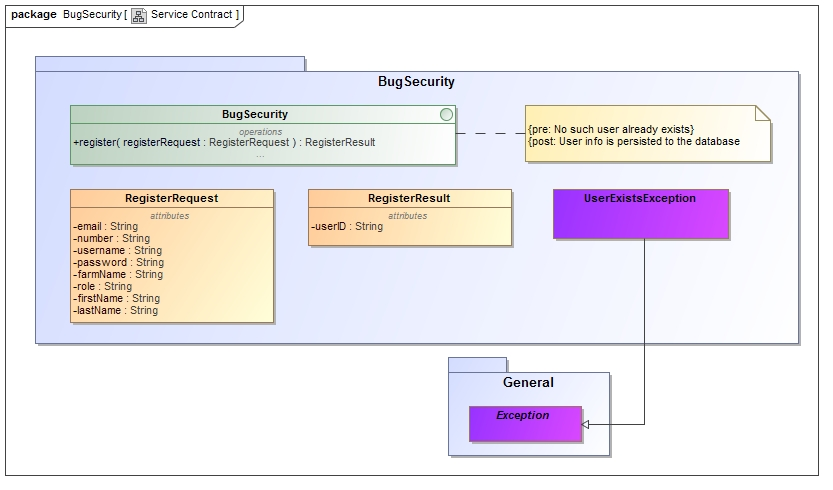
\includegraphics[width=\linewidth]{RegisterSC}		
		
		\paragraph{logout \dotfill [Priority - Medium]}
		This use case provides functionality to log out of the system.\\\hfill\\
		The Service Contract for the \textit{logout} use case is shown below:\\\hfill\\
		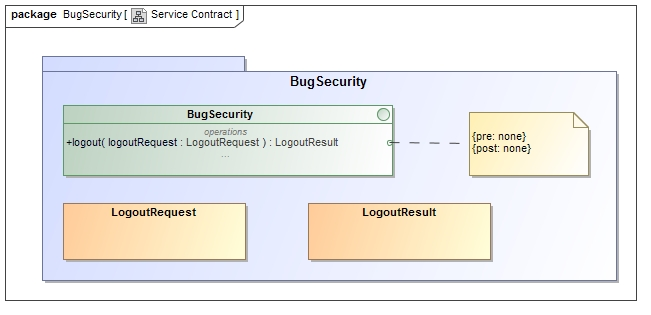
\includegraphics[width=\linewidth]{LogoutSC}
		
		\paragraph{recoverAccount \dotfill [Priority - Low]}
		In the case where a user forgets or has lost his/her credentials to access the system, this use case provides functionality to recover or to generate a new password. User verification is done via the email address associated with the account.\\\hfill\\ 
		The Service Contract for the \textit{recoverAccount} use case is shown below:\\\hfill\\
		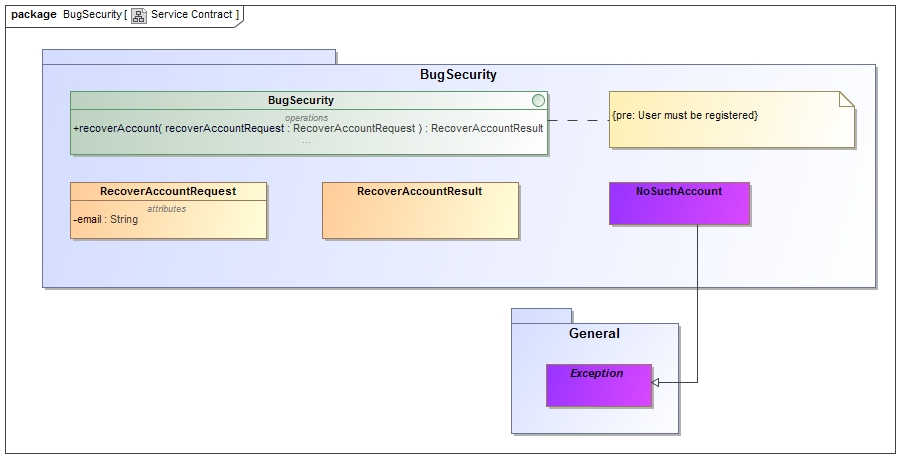
\includegraphics[width=\linewidth]{RecoverAccountSC}
		
		\paragraph{isAuthorised \dotfill [Priority - High]}
		Whenever a service which should not be accessibility to entire plethora of users is requested, authorization is required. This use case makes provision for this.\\\hfill\\
		The Service Contract for the \textit{isAuthorised} use case is shown below:\\\hfill\\
		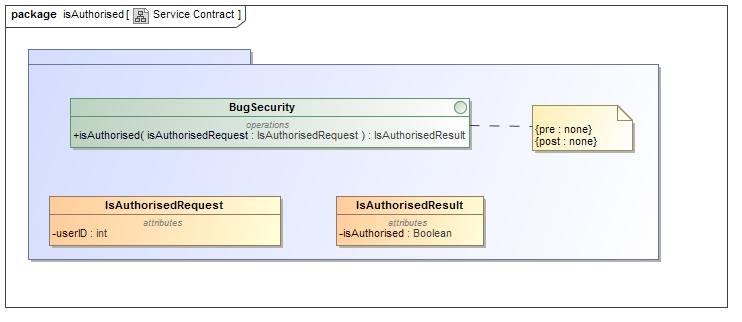
\includegraphics[width=\linewidth]{isAuthorised}
		\paragraph{authoriseUser \dotfill [Priority - Medium]}
		This use case allows for an authorization restriction for a service to be added/\\\hfill\\
		The Service Contract for the \textit{authoriseUser} use case is shown below:\\\hfill\\
		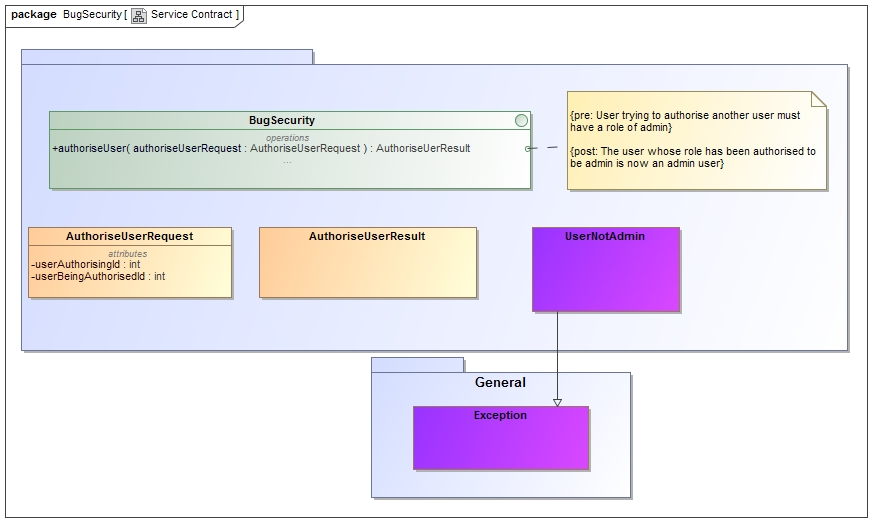
\includegraphics[width=\linewidth]{authorise}
		\paragraph{deauthoriseUser \dotfill [Priority - Medium]}
				This use case allows for an authorization restriction for a service to be removed/\\\hfill\\
		The Service Contract for the \textit{deauthoriseUser} use case is shown below:\\\hfill\\
		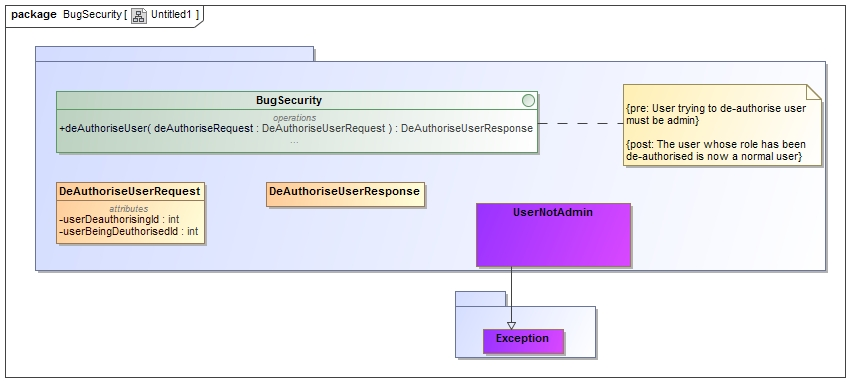
\includegraphics[width=\linewidth]{deauthor}
		
		
		
%------------------------------------------------------------------------------------------%		
	\subsection{BugReporting}
	The BugReporting module allows the following functionality:
	\begin{enumerate}
		\item It provides functionality to generate historical data in a usable, tabular - as used by Microsoft Excel and similar software, format.
		\item It provides functionality to generate a visual representation of historical data in the form of a dynamically chosen set of graphs.
		\item It provides functionality to generate a heat map of the farm with regards to the population of stink bugs identified.
	\end{enumerate}
		\subsubsection{Module Scope}
		The scope of the \textit{BugReporting} module is shown below:\\
		\hfill\\
			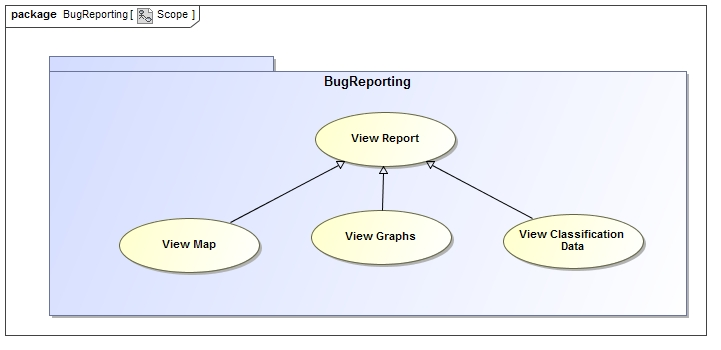
\includegraphics[width=\linewidth]{ReportingScope}
		\subsubsection{Use Cases}
		The concrete use cases for the \textit{BugReporting} module follow:
		\paragraph{viewMap \dotfill [Priority - Medium]}
		This use case provides the functionality to view a heat map, where the total number of pests found will be shown. Areas with more pests will show a darker area on the map. One will this be able to conclude which areas are experiencing a problem with pests. Multiple constraints and filters can be applied to show only a subset of the data available.\\\hfill\\
		The Service Contract for the \textit{viewMap} use case is shown below:\\\hfill\\		
		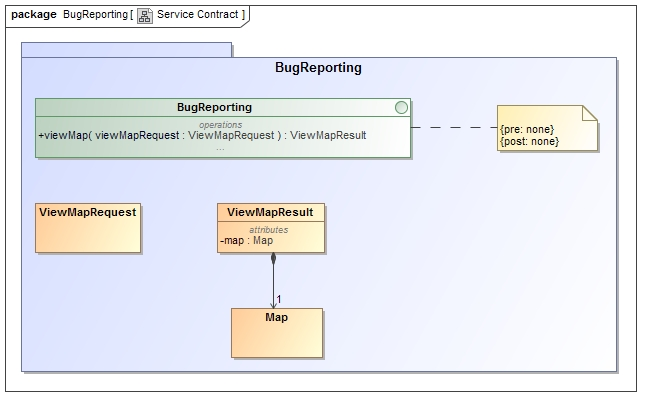
\includegraphics[width=\linewidth]{viewMapSC}
		
		\paragraph{viewCharts \dotfill [Priority - Medium]}
		This use case provides the functionality to view data that was collected through the mobile application, specifically sccouting data. The data will be displayed in the form of dynamic charts, where one can choose multiple filters and constraints to apply to the data. One will be able to see how spraying affects the pest count.\\\hfill\\
		The Service Contract for the \textit{viewCharts} use case is shown below:\\\hfill\\	
		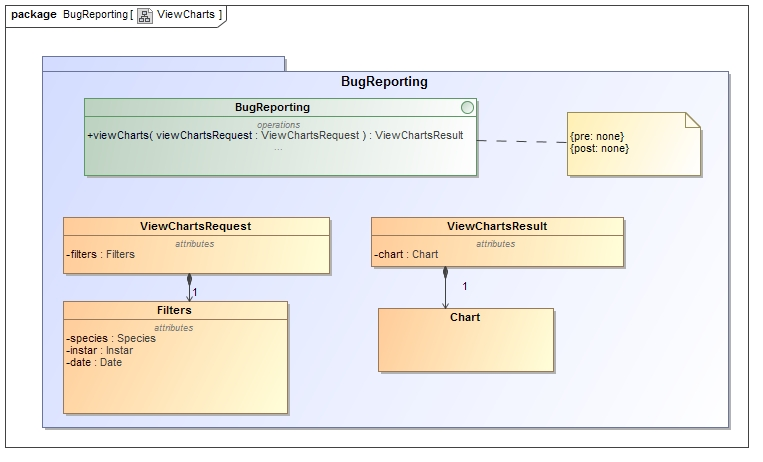
\includegraphics[width=\linewidth]{viewCharts}	
		
		\paragraph{viewTables \dotfill [Priority - Medium]}
		This use case allows the user to see data that has been collected through the mobile application, specifically scouting data. The data will be displayed in the form of a table and will have the functionlity to download this as an Excel spreadsheet, PDF document or to print the table. One will be able to also view spraying data. Multiple filters and constraints can be applied to the data to only view a subset of the data available.\\\hfill\\
		The Service Contract for the \textit{viewTables} use case is shown below:\\\hfill\\
				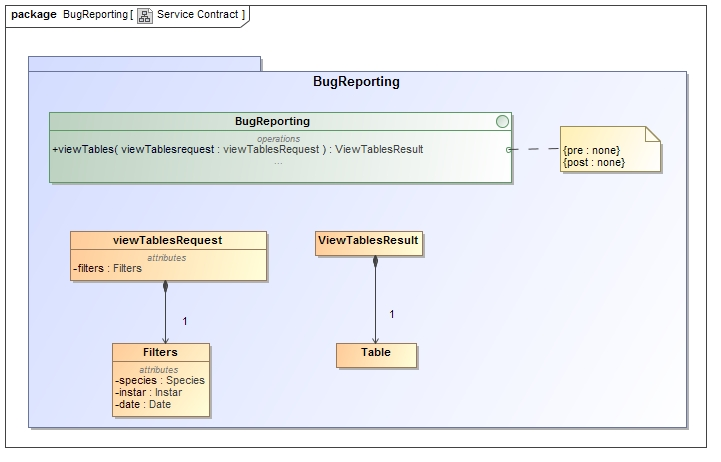
\includegraphics[width=\linewidth]{viewTables}	

	
		

%\section{Open Issues}


%\pagebreak
%\section{Notifications and Messages Domain}
%  \input{Notifications}

\end{document}